\documentclass[a4paper,10pt]{article}

% Encoding.
\usepackage{geometry}
\usepackage[T2A]{fontenc}
\usepackage[utf8]{inputenc}
\usepackage[english,russian]{babel}

\usepackage{hyperref}

\hypersetup{
    colorlinks,
    linkcolor=black,
    urlcolor=blue
}

% Code insertion.
\usepackage[outputdir=build]{minted}

% Math functions.
\usepackage{amsmath}

% Image insertion.
\usepackage{svg}

% No line breaks.
\usepackage[none]{hyphenat}

\title{Задание 4: структурная декомпозиция проекта ``e-гриб''}
\author{
    \begin{tabular}[t]{c@{\extracolsep{8em}}c} 
        Афанасов Артём     & Смирнов Александр \\
        &\\ 
        Струтовский Максим & Федор Жилкин
    \end{tabular}
}

\date{\today}

\begin{document}

\maketitle

% \tableofcontents
% \newpage

\section*{WBS}

Можно приблизить изображение.

    \begin{figure}[h]
        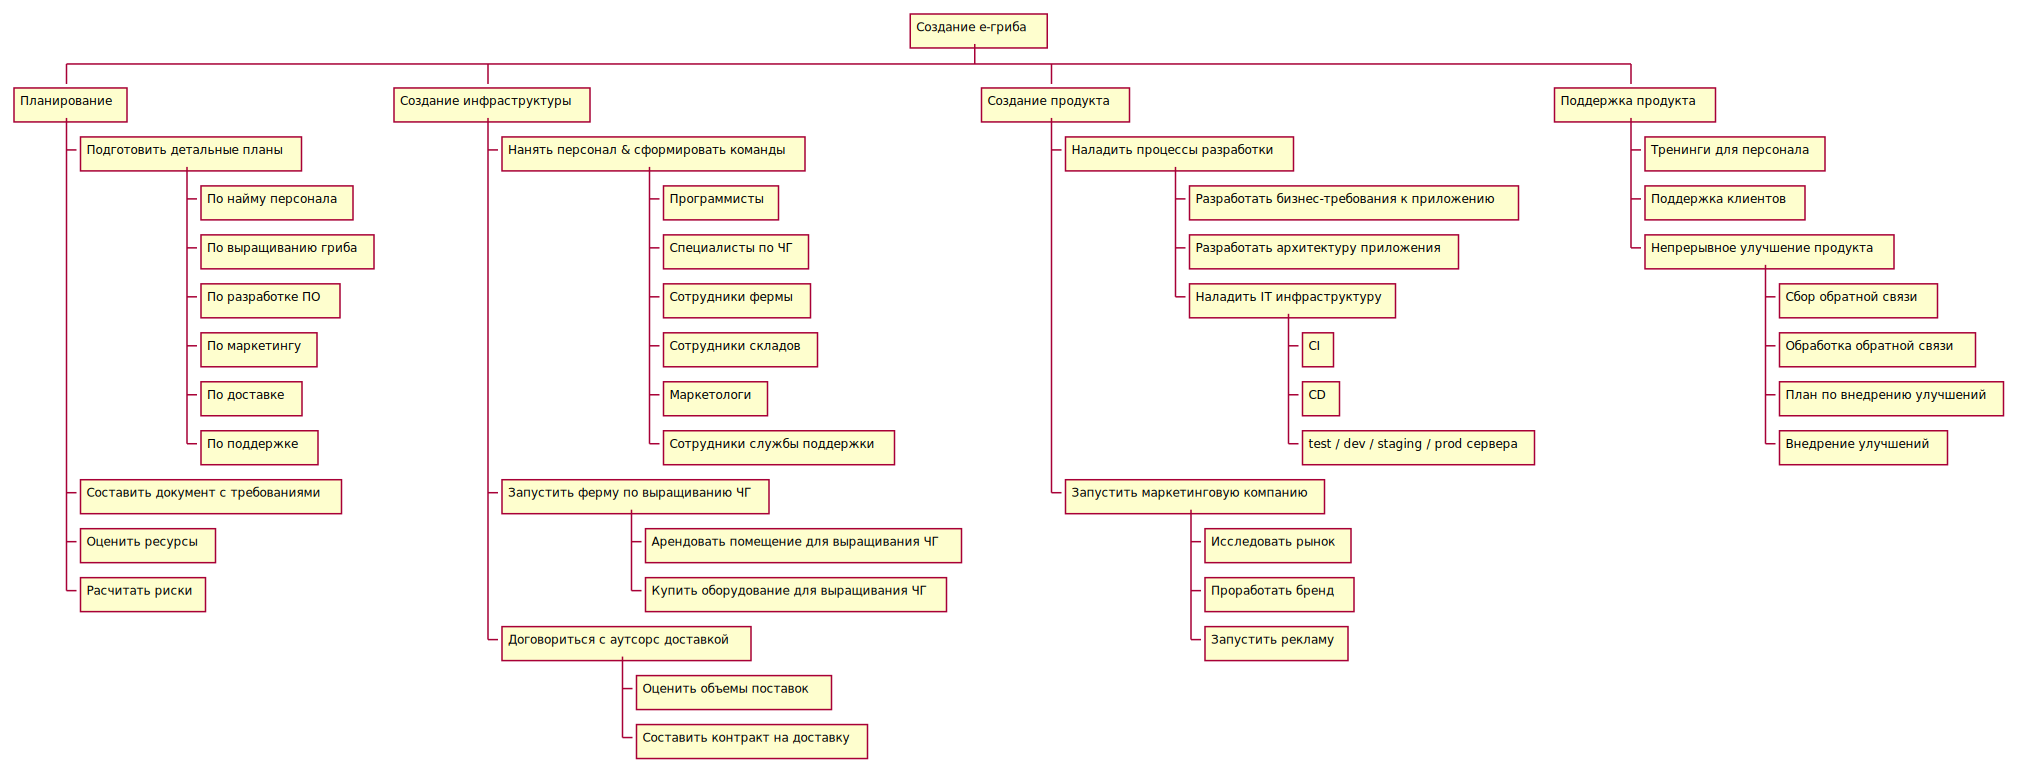
\includegraphics[width=1\textwidth]{./pics/wbs.pdf}
        \centering
    \end{figure}

\end{document}
